\documentclass[11pt,letterpaper]{article}

\usepackage[utf8]{inputenc}
\usepackage[T1]{fontenc}
\usepackage{lmodern}
\usepackage[margin=0.84in,top=0.88in,bottom=0.88in]{geometry}
\usepackage{microtype}
\usepackage{xurl}
\usepackage{amsmath,amssymb}
\usepackage{booktabs}
\usepackage{tabularx}
\usepackage{array}
\usepackage{enumitem}
\usepackage{xcolor}
\usepackage{tcolorbox}
\usepackage{tikz}
\usepackage{pgfplots}
\usepackage{listings}
\usepackage{fancyhdr}
\usepackage{titlesec}
\usepackage{float}
\usepackage{caption}
\usepackage{hyperref}

\pgfplotsset{compat=1.18}
\usetikzlibrary{arrows.meta,positioning,shapes.geometric,fit,backgrounds}

% --- Color Palette (Slate & Deep Navy Engineering Theme) ---
\definecolor{NavyPrimary}{HTML}{0F172A}
\definecolor{BlueAccent}{HTML}{1E3A8A}
\definecolor{SteelSlate}{HTML}{334155}
\definecolor{TealSignal}{HTML}{0F766E}
\definecolor{AmberWarn}{HTML}{B45309}
\definecolor{CrimsonAlert}{HTML}{B91C1C}
\definecolor{SoftBg}{HTML}{F8FAFC}
\definecolor{RuleGray}{HTML}{CBD5E1}

\hypersetup{
    colorlinks=true,
    linkcolor=BlueAccent,
    urlcolor=TealSignal,
    citecolor=BlueAccent,
    pdftitle={Hybrid Load, Endpoint Coverage, and Concurrency Sustainability Testing Methodology for the SD3 Alumni Platform},
    pdfauthor={SD3 Alumni Engineering Team}
}

% --- Typography & Section Styling ---
\titleformat{\section}
  {\Large\bfseries\color{NavyPrimary}}
  {\thesection}{0.8em}{}
  [\vspace{2pt}{\color{RuleGray}\titlerule[0.8pt]}]

\titleformat{\subsection}
  {\large\bfseries\color{BlueAccent}}
  {\thesubsection}{0.7em}{}

\titleformat{\subsubsection}
  {\normalsize\bfseries\color{SteelSlate}}
  {\thesubsubsection}{0.6em}{}

\setlist[itemize]{leftmargin=1.4em,itemsep=2pt,topsep=4pt}
\setlist[enumerate]{leftmargin=1.6em,itemsep=3pt,topsep=4pt}
\setlength{\emergencystretch}{2.5em}
\tolerance=1200

% --- Running Headers / Footers ---
\pagestyle{fancy}
\fancyhf{}
\fancyhead[L]{\small\color{SteelSlate}\textbf{SD3 Alumni Platform} --- Testing Methodology White Paper}
\fancyhead[R]{\small\color{SteelSlate}Target: \texttt{https://najealp.top}}
\fancyfoot[L]{\small\color{SteelSlate}Document Revision 2.0 \quad|\quad November 11, 2026}
\fancyfoot[R]{\small\color{SteelSlate}Page \thepage}
\renewcommand{\headrulewidth}{0.4pt}
\renewcommand{\footrulewidth}{0.4pt}

% --- Callout Boxes ---
\tcbuselibrary{breakable}
\newtcolorbox{calloutbox}[2][BlueAccent]{
  colback=SoftBg,
  colframe=#1,
  coltitle=white,
  fonttitle=\bfseries\small,
  title=#2,
  arc=3pt,
  boxrule=0.9pt,
  left=8pt,
  right=8pt,
  top=6pt,
  bottom=6pt,
  breakable
}

% --- Code Listings ---
\lstset{
  basicstyle=\ttfamily\footnotesize,
  backgroundcolor=\color{SoftBg},
  frame=single,
  rulecolor=\color{RuleGray},
  breaklines=true,
  breakatwhitespace=true,
  showstringspaces=false,
  tabsize=2,
  keywordstyle=\bfseries\color{BlueAccent},
  commentstyle=\itshape\color{TealSignal},
  stringstyle=\color{AmberWarn},
  xleftmargin=4pt,
  xrightmargin=4pt
}

\begin{document}

% ==============================================================================
% TITLE HEADER
% ==============================================================================
\thispagestyle{empty}
\begin{tcolorbox}[
  colback=NavyPrimary,
  colframe=NavyPrimary,
  arc=4pt,
  left=16pt,
  right=16pt,
  top=18pt,
  bottom=18pt
]
  {\color{RuleGray}\small\textsc{Engineering White Paper \quad|\quad Performance, Coverage \& Sustainability Validation}}\\[6pt]
  {\color{white}\LARGE\bfseries Hybrid Load, Endpoint Coverage, and SQLite\\Concurrency Testing Methodology for SD3 Alumni}\\[10pt]
  {\color{RuleGray}\normalsize
  A Pre-Seeded, Two-Phase Orchestration Architecture Combining Deterministic SQL\\
  Provisioning, Fail-Fast JMeter Contract Verification, Stepped Concurrency up to\\
  1,000 Virtual Users, Behavioral Locust Personas, and Automated Reporting}
\end{tcolorbox}

\vspace{6pt}
\noindent\begin{tabularx}{\textwidth}{@{} >{\raggedright\arraybackslash}p{0.23\textwidth} >{\raggedright\arraybackslash}p{0.26\textwidth} >{\raggedright\arraybackslash}p{0.28\textwidth} >{\raggedright\arraybackslash}X @{}}
  \textbf{Target Environment:} & \textbf{Database Engine:} & \textbf{Uplink Envelope:} & \textbf{Effective Date:} \\
  \texttt{https://najealp.top} & SQLite (\texttt{DELETE} mode) & $70\text{ Mbps}$ ($\approx 8.75\text{ MB/s}$) & November 11, 2026 \\
\end{tabularx}
\vspace{8pt}
{\color{RuleGray}\hrule height 1pt}
\vspace{10pt}

\begin{abstract}
\noindent Conventional API stress tests frequently mischaracterize production readiness because of three methodological failures: silent HTTP \texttt{401 Unauthorized} cascades that inflate synthetic throughput without exercising database paths, unpaced burst loops whose samples collapse to start/end boundaries of time-series charts, and homogeneous read-only requests that overlook connection queuing and database lock contention. This white paper formalizes the deterministic load and sustainability methodology implemented for the SD3 Alumni platform (\texttt{test/load/}). Beginning with a repeatable pre-test SQL provisioning script (\texttt{test/load/hell.sql}) that snapshots SQLite \texttt{dev.db}, seeds multi-role accounts alongside moderation/RSVP targets, and normalizes credentials, the pipeline executes a fail-fast \textbf{Phase~1} pre-flight credential check and 186-sampler CRUD coverage gate ($191$ total requests) in Apache JMeter (\texttt{benchmark.jmx}), followed by a \textbf{Phase~2} stepped capacity sweep ($100\to 1{,}000$ VUs, run standalone via \texttt{run\_jmeter.ps1} or concurrently with stateful Locust personas via \texttt{run\_parallel\_suite.ps1}), and concluding with \textbf{Phase~3} automated HTML, Excel, and PDF telemetry synthesis (\texttt{generate\_report.py} and \texttt{export\_reports\_pdf.mjs}). Full five-tier empirical verification against \texttt{https://najealp.top} (\texttt{test/load/results/jmeter\_report.pdf}, 17:41--17:44 local time) recorded \textbf{$0.00\%$ HTTP failure} and \textbf{$0$ HTTP \texttt{401}/\texttt{403}/\texttt{5xx} responses} across \textbf{$23{,}157$ total requests} ($191$ pre-flight/coverage + $22{,}966$ load samples, including $2$ HTTP~\texttt{304} cache hits), achieving an aggregate \textbf{$\text{APDEX} = 0.970$} ($95.06\%$ $\le 500\text{ ms}$), overall $p_{50} = 73.00\text{ ms}$, $p_{95} = 566.00\text{ ms}$, $p_{99} = 1577.93\text{ ms}$, and peak Tier~5 throughput of $192.90\text{ req/s}$ ($10.07\text{ Mbps}$ mean; $291\text{ req/s}$ 1-s HTML dashboard peak). Tier-by-tier telemetry confirms nearly flat response latency from $100$ through $750$ VUs ($p_{50} = 70\text{--}72\text{ ms}$, $p_{95} = 220\text{--}248\text{ ms}$, $\text{APDEX} \ge 0.998$) after Nginx HTTP/2 keep-alive, asynchronous \texttt{bcryptjs}, in-memory ETag/TTL caching, Prisma indexing, and payload slimming optimizations, while isolating a transient TLS/socket handshake queue during the $750\to 1{,}000$-VU ramp transition that recovers cleanly under full $1{,}000$-VU load.
\end{abstract}

\vspace{6pt}
\tableofcontents
\vspace{8pt}
{\color{RuleGray}\hrule height 0.6pt}

% ==============================================================================
% SECTION 1
% ==============================================================================
\section{System Under Test and Operational Envelope}

\subsection{Application Stack and Persistence Layer}
The SD3 Alumni platform exposes a reverse-proxied monolithic Node.js backend (\texttt{api/index.js}) serving JSON REST routes and a compiled React~19 Single-Page Application (SPA) catch-all handler:
\begin{itemize}
  \item \textbf{Reverse Proxy \& Keep-Alive Envelope (\texttt{nginx/nginx.conf}, \texttt{nginx/alumni.conf}):} Public HTTPS traffic terminates at Nginx with HTTP/2 enabled (\texttt{http2 on}), \texttt{worker\_rlimit\_nofile 65535}, \texttt{worker\_connections 4096}, \texttt{keepalive\_timeout 65}, gzip compression (\texttt{gzip\_comp\_level 5}, \texttt{min\_length 1024}), upstream connection pooling (\texttt{upstream alumni\_api \{ keepalive 256; \}}), and direct static asset serving for \texttt{/images/} and \texttt{/uploads/} with 7-day cache headers. Node.js matches this keep-alive window explicitly via \texttt{server.keepAliveTimeout = 65000} and \texttt{server.headersTimeout = 66000}.
  \item \textbf{HTTP Routing \& JWT Authentication:} Express~5 (\texttt{express \^{}5.3.0}) enforces JWT authentication (\texttt{jsonwebtoken \^{}9.0.3}) supporting extraction from \texttt{Authorization: Bearer} headers and HTTP cookies (\texttt{token} / \texttt{adminToken}). Role separation rejects unauthenticated callers with HTTP~\texttt{401} and non-user/admin mismatches with HTTP~\texttt{403} via \texttt{authenticateToken} and \texttt{authenticateAdminToken}.
  \item \textbf{ORM, Indexing \& List Payload Slimming:} Prisma ORM (\texttt{@prisma/client \^{}7.10.1}) binds via \texttt{@prisma/adapter-better-sqlite3} to native \texttt{better-sqlite3} (\texttt{\^{}12.11.1}), backed by \textbf{33 explicit \texttt{@@index} declarations} in \texttt{prisma/schema.prisma}. Generic REST routes (\texttt{GET/\allowbreak POST/\allowbreak PATCH/\allowbreak PUT/\allowbreak DELETE /api/:table}) share dynamic filtering, sorting, and relational hydration via \texttt{queryParser.js} (\texttt{\_where}, \texttt{\_sort}, \texttt{\_order}, \texttt{\_include}, \texttt{\_page}, \texttt{\_per\_page}), while \texttt{defaultListIncludes} in \texttt{api/index.js} constrains default list-view joins so paginated JSON feeds average $12\text{--}15\text{ KB/req}$ (down from $\approx 85\text{ KB/req}$ prior to Tier-3 tuning).
  \item \textbf{Asynchronous Cryptography \& Multi-Tier In-Memory Caching:} Password hashing and verification (\texttt{bcryptjs \^{}3.0.3}, cost factor $10$) execute strictly asynchronously (\texttt{await bcrypt.compare(...)} and \texttt{await bcrypt.hash(..., 10)}; zero blocking \texttt{hashSync}/\texttt{compareSync} calls remain in \texttt{api/index.js}). Read hot paths leverage three bounded in-memory caches emitting weak ETags (\texttt{W/"..."}) and HTTP \texttt{304 Not Modified} responses: \texttt{feedCache} ($60\text{ s}$ default TTL for \texttt{/api/bulletins} and \texttt{/api/events}), \texttt{lookupCache} ($300\text{ s}$ TTL for 10 reference tables), and \texttt{adminDashboardStatsCache} ($20\text{ s}$ TTL with single-flight \texttt{adminDashboardStatsInFlight} stampede deduplication), all invalidated automatically on mutations via \texttt{invalidateRelatedCaches}.
  \item \textbf{Media, Gateways \& Rate Limiters:} Image uploads process through \texttt{multer} and \texttt{sharp} (\texttt{POST /\allowbreak api/\allowbreak upload}); donations integrate PayMongo (\texttt{POST /\allowbreak api/\allowbreak donations/\allowbreak checkout} and \texttt{/\allowbreak api/\allowbreak donations/\allowbreak webhook}). During benchmark campaigns, \texttt{authLimiter} and \texttt{contentLimiter} (\texttt{express-rate-limit}) bypass throttling (\texttt{skip: () => true}) to expose underlying server and transport limits.
\end{itemize}

\subsection{Deliberate SQLite Journal Policy and Physical Bandwidth Ceiling}
Per project architectural constraints (\texttt{api/index.js}), the database explicitly maintains rollback journal mode rather than Write-Ahead Logging:
\begin{lstlisting}[language=SQL,caption={Active SQLite concurrency pragmas initialized at backend startup (\texttt{api/index.js}).}]
PRAGMA journal_mode = DELETE;
PRAGMA busy_timeout = 10000;
\end{lstlisting}
In \texttt{DELETE} mode, SQLite permits concurrent shared reads when no writer commits, but acquiring an exclusive commit lock blocks all concurrent readers and writers until the rollback journal is unlinked, bounded by the $10\text{ s}$ adapter and SQLite \texttt{busy\_timeout}. Preserving this constraint intentionally lets test suites measure lock-queue behavior realistically rather than masking it.

Simultaneously, \texttt{test/load/config.json} models the target VPS host under a physical network ceiling of $C_{\text{uplink}} = 70\text{ Mbits/s}$ ($\approx 8.75\text{ MB/s}$). For HTTP responses with average wire payload $\bar{S}$ bytes, the theoretical network-bound request ceiling $\lambda_{\max}$ satisfies:
\begin{equation}
  \label{eq:bandwidth}
  \lambda_{\max} = \frac{C_{\text{uplink}} \times 10^{6}}{8 \cdot \bar{S}} \quad \text{[req/s]}.
\end{equation}
Prior to list-payload slimming, heavy paginated feeds averaging $\bar{S} \approx 85\text{ KB}$ risked link saturation around $103\text{ req/s}$. With Tier-3 \texttt{defaultListIncludes} slimming and Nginx gzip compression bringing paginated catalogs to $12\text{--}15\text{ KB/req}$ (and the blended 51-route JMeter load mix to $\bar{S} = 6.34\text{ KB/req}$), $\lambda_{\max}$ expands above $580\text{--}1{,}380\text{ req/s}$, ensuring bandwidth does not bottleneck concurrency below $1{,}000$ VUs.

% ==============================================================================
% SECTION 2
% ==============================================================================
\section{Methodological Foundations and Threat Model}

During suite evolution, three structural pathologies of naive load tests were identified and systematically eliminated:

\begin{enumerate}
  \item \textbf{The Silent \texttt{401} Throughput Mirage:} If seeded accounts or JWT tokens fail before load generation, protected routes short-circuit in middleware before touching Prisma or SQLite. Throughput rises artificially while real application logic remains untested. Our methodology requires deterministic database pre-seeding (\texttt{test/load/hell.sql}) plus automated setup token verification, treating \emph{any} \texttt{HTTP 401} across Phase~1 or Phase~2 as a hard suite failure (exit code \texttt{2}).
  \item \textbf{Edge-Hugging Time-Series Collapse ("Request Slamming"):} Closed-loop threads lacking inter-request think times dispatch requests simultaneously at thread spawn and finish together before sampling intervals settle. With JMeter's default $60\text{ s}$ HTML report granularity and zero timer delay, time-series charts collapse to left/right edge points. Introducing randomized per-iteration \texttt{UniformRandomTimer} pacing ($\mathcal{U}(1500, 4000)\text{ ms}$ in Full \texttt{config.json} defaults; $\mathcal{U}(100, 500)\text{ ms}$ in early micro-benchmarks), setting \texttt{overall\_granularity = 1000 ms}, and filtering setup/coverage rows out of load telemetry restores physically faithful per-second waveforms.
  \item \textbf{Cross-VU State Collisions:} When multiple virtual users target identical primary keys for RSVPs, social connections, or moderation toggles, unique constraints and state-transition races distort error rates with test-harness artifacts rather than genuine server faults. We isolate state via pre-provisioned multi-account pools, VU-owned disposable resources, dedicated moderation target pools, and deterministic snapshot rollback.
\end{enumerate}

\begin{calloutbox}[TealSignal]{Execution Modes: Standalone Stepped Capacity vs.\ Hybrid Read/Write Personas}
The repository supports three complementary execution modes tailored to distinct engineering questions: (1)~the legacy unpaced Node.js worker probe (\texttt{test/load/node\_benchmark.js}) across $20$ read routes for baseline socket/WAN ceilings; (2)~standalone five-tier JMeter stepped capacity verification (\texttt{run\_jmeter.ps1 -HtmlReport -ExcelReport -PdfReport}) driving $100\to 1{,}000$ VUs across $51$ probability-weighted routes to certify latency/APDEX scaling and publish the 4-page HTML/PDF dashboard (\texttt{jmeter\_report.pdf}) plus 5-sheet Excel workbook (\texttt{jmeter\_stress\_test\_report.xlsx}); and (3)~unified parallel orchestration (\texttt{run\_parallel\_suite.ps1}) layering stateful write-heavy Locust personas on top of stepped JMeter load to stress \texttt{DELETE}-mode write serialization simultaneously.
\end{calloutbox}

% ==============================================================================
% SECTION 3
% ==============================================================================
\section{Two-Phase Orchestration Architecture}

Figure~\ref{fig:architecture} illustrates the full test pipeline orchestrated from \texttt{test/load/}, enforcing Python environment validation (\texttt{.agents/python.md}), deterministic database state, fail-fast functional gating, and multi-artifact reporting.

\begin{figure}[H]
\centering
\resizebox{\linewidth}{!}{%
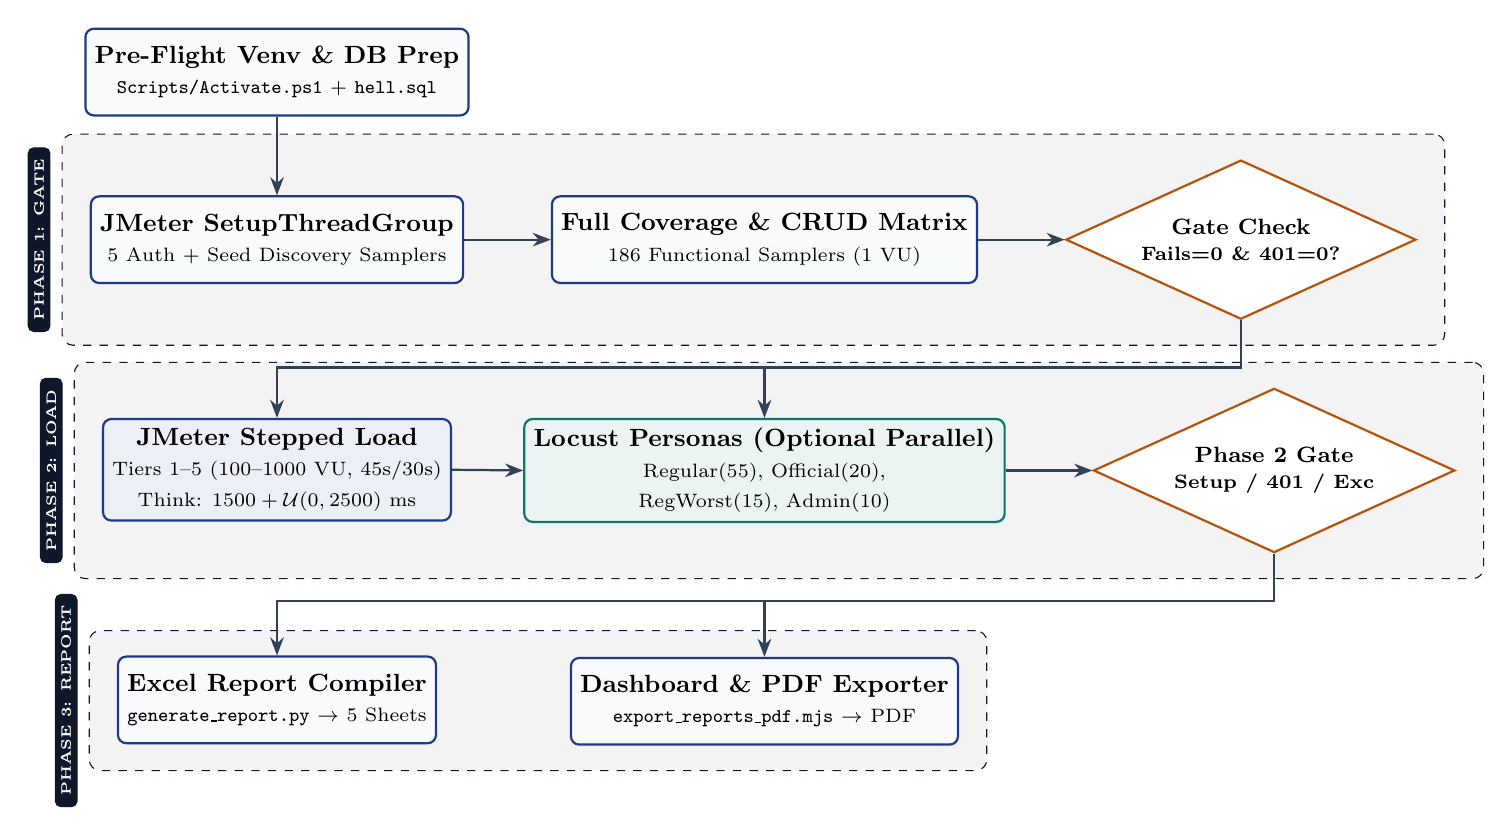
\begin{tikzpicture}[
  node distance=18mm and 11mm,
  box/.style={draw=BlueAccent, fill=SoftBg, rounded corners=3pt, thick, minimum width=3.85cm, minimum height=1.1cm, align=center, font=\small},
  gate/.style={draw=AmberWarn, fill=white, diamond, aspect=2.2, thick, align=center, font=\footnotesize\bfseries},
  phase/.style={draw=NavyPrimary, fill=NavyPrimary!5, rounded corners=4pt, dashed, inner xsep=10pt, inner ysep=9pt},
  lane/.style={draw=NavyPrimary, fill=NavyPrimary, text=white, font=\tiny\bfseries, rounded corners=2pt, rotate=90, anchor=south, inner xsep=4pt, inner ysep=2.2pt},
  arrow/.style={-{Stealth[length=2.3mm]}, thick, color=SteelSlate}
]

% Env & SQL Prep
\node[box] (venv) {\textbf{Pre-Flight Venv \& DB Prep}\\{\scriptsize \texttt{Scripts/Activate.ps1} + \texttt{hell.sql}}};

% Phase 1
\node[box, below=10mm of venv] (p1setup) {\textbf{JMeter SetupThreadGroup}\\{\scriptsize 5 Auth + Seed Discovery Samplers}};
\node[box, right=11mm of p1setup] (p1cov) {\textbf{Full Coverage \& CRUD Matrix}\\{\scriptsize 186 Functional Samplers (1 VU)}};
\node[gate, right=11mm of p1cov] (p1gate) {Gate Check\\{\scriptsize Fails=0 \& 401=0?}};

% Phase 2 parallel
\node[box, below=17mm of p1setup, fill=BlueAccent!8] (p2jm) {\textbf{JMeter Stepped Load}\\{\scriptsize Tiers 1--5 ($100\text{--}1000$ VU, $45\text{s}$/$30\text{s}$)}\\{\scriptsize Think: $1500 + \mathcal{U}(0,2500)\text{ ms}$}};
\node[box, below=17mm of p1cov, fill=TealSignal!8, draw=TealSignal] (p2loc) {\textbf{Locust Personas (Optional Parallel)}\\{\scriptsize Regular(55), Official(20),}\\{\scriptsize RegWorst(15), Admin(10)}};
\node[gate, right=11mm of p2loc] (p2gate) {Phase 2 Gate\\{\scriptsize Setup / 401 / Exc}};

% Phase 3
\node[box, below=17mm of p2jm] (p3xl) {\textbf{Excel Report Compiler}\\{\scriptsize \texttt{generate\_report.py} $\to$ 5 Sheets}};
\node[box, below=17mm of p2loc] (p3pdf) {\textbf{Dashboard \& PDF Exporter}\\{\scriptsize \texttt{export\_reports\_pdf.mjs} $\to$ PDF}};

% Backgrounds + unobstructed vertical swimlane pills
\begin{scope}[on background layer]
  \node[phase, fit=(p1setup)(p1cov)(p1gate)] (bg1) {};
  \node[phase, fit=(p2jm)(p2loc)(p2gate)] (bg2) {};
  \node[phase, fit=(p3xl)(p3pdf)] (bg3) {};
  \node[lane] at ([xshift=-4pt]bg1.west) {PHASE 1: GATE};
  \node[lane] at ([xshift=-4pt]bg2.west) {PHASE 2: LOAD};
  \node[lane] at ([xshift=-4pt]bg3.west) {PHASE 3: REPORT};
\end{scope}

% Arrows
\draw[arrow] (venv.south) -- (p1setup.north);
\draw[arrow] (p1setup) -- (p1cov);
\draw[arrow] (p1cov) -- (p1gate);
\draw[arrow] (p1gate.south) -- ++(0,-6mm) coordinate (junc1) -| (p2loc.north);
\draw[arrow] (junc1) -| (p2jm.north);
\draw[arrow] (p2jm.east) -- (p2loc.west);
\draw[arrow] (p2loc.east) -- (p2gate.west);
\draw[arrow] (p2gate.south) -- ++(0,-6mm) coordinate (junc2) -| (p3pdf.north);
\draw[arrow] (junc2) -| (p3xl.north);

\end{tikzpicture}%
}
\caption{End-to-end orchestration pipeline across \texttt{test/load/}. Phase~0/1 prepares \texttt{dev.db} via \texttt{hell.sql} and gates Phase~2 behind a 191-sampler auth/CRUD pass; Phase~2 runs stepped JMeter load ($100\to 1{,}000$ VUs) standalone (\texttt{run\_jmeter.ps1}) or alongside Locust (\texttt{run\_parallel\_suite.ps1}); Phase~3 generates 5-sheet Excel workbooks and Chromium-rendered PDF reports (\texttt{jmeter\_report.pdf} or unified \texttt{load\_test\_report.pdf}).}
\label{fig:architecture}
\end{figure}

Before invoking Python utilities or Locust, \texttt{run\_parallel\_suite.ps1} and \texttt{run\_jmeter.ps1} validate the repository-local virtual environment: activating \texttt{Scripts/\allowbreak Activate.ps1}, asserting \texttt{\$env:VIRTUAL\_ENV} matches the repository root, verifying \texttt{python} resolves to \texttt{Scripts/\allowbreak python.exe}, and confirming \texttt{sys.prefix != \allowbreak sys.base\_prefix} per \texttt{.agents/\allowbreak python.md}. Stale JTL, JSON, log, and HTML output artifacts in \texttt{test/load/results/} are purged prior to execution.

% ==============================================================================
% SECTION 4
% ==============================================================================
\section{Pre-Test Database Provisioning and Phase~1 Coverage Gate}

\subsection{Pre-Test SQLite State Provisioning (\texttt{test/load/hell.sql})}
High-concurrency test campaigns cannot rely solely on on-the-fly API registration when multi-role connection pools ($10$ Administrators, $5$ Official alumni, and $5$ Regular alumni) must sign tokens immediately during the Phase~1 setup step without triggering registration write storms or hitting empty moderation/RSVP queues. Prior to executing the benchmark suite against \texttt{https://najealp.top}, operators execute \texttt{test/load/hell.sql} directly against the SQLite \texttt{dev.db} database on the VPS host:
\begin{enumerate}
  \item \textbf{Pre-Stress Binary Snapshot (Step~1):} Operators take a timestamped binary copy of \texttt{dev.db} (\texttt{cp dev.db dev.db.bak\_pre\_stress\_\$(date +\%s)}) prior to applying SQL mutations, establishing an instantaneous byte-exact restore point.
  \item \textbf{Deterministic Multi-Role Pool Upserts (Steps~2--4):} Idempotent SQL statements seed or refresh $10$ Admin accounts (\texttt{adm-loadtest-01} through \texttt{adm-loadtest-10}, usernames \texttt{admin1}--\texttt{admin10} via \texttt{ON CONFLICT(username) DO UPDATE}), $5$ verified Official members (\texttt{usr-off-01}--\texttt{usr-off-05}, \texttt{userStatusId = 'OWOyGJzHfV'}), and $5$ Regular members (\texttt{usr-reg-01}--\texttt{usr-reg-05}, \texttt{userStatusId = '2Ue2cfwVMa'}) across \texttt{User}, \texttt{UserAuth}, public \texttt{Profile} (\texttt{kvf-XCOljU}), and \texttt{UserStatistic}, all bound to a pre-computed \texttt{bcrypt} cost-$10$ hash for password \texttt{123456}.
  \item \textbf{Moderation \& Active RSVP Targets (Step~5):} Seeds $5$ Pending bulletins (\texttt{blt-pending-01}--\texttt{05}, \texttt{contentStatusId = 'a6ze5OaKs0'}), $2$ Pending events (\texttt{evt-pending-01}--\texttt{02}, \texttt{eventStatusId = 'G0sRtXA38I'}), and $2$ Approved RSVP events (\texttt{evt-active-rsvp-01}--\texttt{02}, \texttt{eventStatusId = 'j3Ua4WQwdl'}) using \texttt{COALESCE} category lookups so admin moderation and high-concurrency RSVP paths always locate valid targets.
  \item \textbf{Global Staging Credential Normalization (Step~6):} Updates \texttt{passwordHash} across all rows in \texttt{UserAuth} and \texttt{Admin} to \texttt{\$2a\$10\$LBJk5tBWm6IWAbNmeArmaeRHtMnDsnKsofbUbiWrbSrpMgqn5C29O} (password \texttt{123456}) so load engines can authenticate arbitrary existing staging accounts seamlessly without \texttt{401} rejections. Because this step irreversibly overwrites prior password digests, Step~1 backup capture and post-test restoration are mandatory.
\end{enumerate}

Listing~\ref{lst:hell_sql} reproduces the complete pre-test SQL initialization script executed before the benchmark campaign.

\begin{lstlisting}[language=SQL,basicstyle=\ttfamily\fontsize{6.4}{7.6}\selectfont,commentstyle=\color{TealSignal},numbers=left,numberstyle=\tiny\color{SteelSlate},breaklines=true,breakatwhitespace=false,keepspaces=true,caption={Complete pre-test SQLite setup script (\texttt{test/load/hell.sql}) executed prior to load testing.},label={lst:hell_sql}]
-- ==============================================================================
-- PRE-TEST DATABASE SETUP SCRIPT FOR HIGH-CONCURRENCY LOAD TESTING
-- Target: https://najealp.top (dev.db SQLite Database)
-- Password for all generated test accounts: 123456
-- Bcrypt Hash (cost 10): $2b$10$OWJFhm7ALzwkqTNSmE0qYO0hwTnHlGLAG8s5qAMmfqvhHozxa4ZzW
-- ==============================================================================
--
-- ------------------------------------------------------------------------------
-- STEP 1: VPS SAFETY BACKUP
-- Run this in bash on the VPS BEFORE running this SQL file:
--   cp dev.db dev.db.bak_pre_stress_$(date +%s)
-- ------------------------------------------------------------------------------

-- ------------------------------------------------------------------------------
-- STEP 2: PROVISION 10 DEDICATED ADMINISTRATORS
-- Usernames: admin1 through admin10 | Password: "123456"
-- ------------------------------------------------------------------------------
INSERT INTO Admin (id, username, passwordHash, lastLogin)
VALUES 
    ('adm-loadtest-01', 'admin1', '$2b$10$OWJFhm7ALzwkqTNSmE0qYO0hwTnHlGLAG8s5qAMmfqvhHozxa4ZzW', CURRENT_TIMESTAMP),
    ('adm-loadtest-02', 'admin2', '$2b$10$OWJFhm7ALzwkqTNSmE0qYO0hwTnHlGLAG8s5qAMmfqvhHozxa4ZzW', CURRENT_TIMESTAMP),
    ('adm-loadtest-03', 'admin3', '$2b$10$OWJFhm7ALzwkqTNSmE0qYO0hwTnHlGLAG8s5qAMmfqvhHozxa4ZzW', CURRENT_TIMESTAMP),
    ('adm-loadtest-04', 'admin4', '$2b$10$OWJFhm7ALzwkqTNSmE0qYO0hwTnHlGLAG8s5qAMmfqvhHozxa4ZzW', CURRENT_TIMESTAMP),
    ('adm-loadtest-05', 'admin5', '$2b$10$OWJFhm7ALzwkqTNSmE0qYO0hwTnHlGLAG8s5qAMmfqvhHozxa4ZzW', CURRENT_TIMESTAMP),
    ('adm-loadtest-06', 'admin6', '$2b$10$OWJFhm7ALzwkqTNSmE0qYO0hwTnHlGLAG8s5qAMmfqvhHozxa4ZzW', CURRENT_TIMESTAMP),
    ('adm-loadtest-07', 'admin7', '$2b$10$OWJFhm7ALzwkqTNSmE0qYO0hwTnHlGLAG8s5qAMmfqvhHozxa4ZzW', CURRENT_TIMESTAMP),
    ('adm-loadtest-08', 'admin8', '$2b$10$OWJFhm7ALzwkqTNSmE0qYO0hwTnHlGLAG8s5qAMmfqvhHozxa4ZzW', CURRENT_TIMESTAMP),
    ('adm-loadtest-09', 'admin9', '$2b$10$OWJFhm7ALzwkqTNSmE0qYO0hwTnHlGLAG8s5qAMmfqvhHozxa4ZzW', CURRENT_TIMESTAMP),
    ('adm-loadtest-10', 'admin10', '$2b$10$OWJFhm7ALzwkqTNSmE0qYO0hwTnHlGLAG8s5qAMmfqvhHozxa4ZzW', CURRENT_TIMESTAMP)
ON CONFLICT(username) DO UPDATE SET 
    passwordHash = excluded.passwordHash,
    lastLogin = CURRENT_TIMESTAMP;

-- ------------------------------------------------------------------------------
-- STEP 3: PROVISION 5 VERIFIED OFFICIAL TEST USERS
-- Emails: test.official1@najealp.top to test.official5@najealp.top | Password: "123456"
-- Status: Official ('OWOyGJzHfV') | Profile: Public ('kvf-XCOljU')
-- ------------------------------------------------------------------------------

-- User 1 (Official)
INSERT OR REPLACE INTO User (id, userStatusId, profileStatusId)
VALUES ('usr-off-01', 'OWOyGJzHfV', 'kvf-XCOljU');
INSERT OR REPLACE INTO UserAuth (userId, email, passwordHash, lastLogin)
VALUES ('usr-off-01', 'test.official1@najealp.top', '$2b$10$OWJFhm7ALzwkqTNSmE0qYO0hwTnHlGLAG8s5qAMmfqvhHozxa4ZzW', CURRENT_TIMESTAMP);
INSERT OR REPLACE INTO Profile (userId, userName, gender, bio, email, degreeId, batch)
VALUES ('usr-off-01', 'Official Tester One', 'Female', 'Verified Official Load Test Account', 'test.official1@najealp.top', 'hd2F5ini8q', 2022);
INSERT OR REPLACE INTO UserStatistic (userId, userConnections, eventsAttended, eventsCreated, bulletinsCreated, commentsWritten, achievements, donatedAmount, dateRegistered)
VALUES ('usr-off-01', 5, 2, 5, 3, 10, 2, 500.0, CURRENT_TIMESTAMP);

-- User 2 (Official)
INSERT OR REPLACE INTO User (id, userStatusId, profileStatusId)
VALUES ('usr-off-02', 'OWOyGJzHfV', 'kvf-XCOljU');
INSERT OR REPLACE INTO UserAuth (userId, email, passwordHash, lastLogin)
VALUES ('usr-off-02', 'test.official2@najealp.top', '$2b$10$OWJFhm7ALzwkqTNSmE0qYO0hwTnHlGLAG8s5qAMmfqvhHozxa4ZzW', CURRENT_TIMESTAMP);
INSERT OR REPLACE INTO Profile (userId, userName, gender, bio, email, degreeId, batch)
VALUES ('usr-off-02', 'Official Tester Two', 'Male', 'Verified Official Load Test Account', 'test.official2@najealp.top', 'GISquVZHHs', 2021);
INSERT OR REPLACE INTO UserStatistic (userId, userConnections, eventsAttended, eventsCreated, bulletinsCreated, commentsWritten, achievements, donatedAmount, dateRegistered)
VALUES ('usr-off-02', 4, 1, 3, 2, 8, 1, 250.0, CURRENT_TIMESTAMP);

-- User 3 (Official)
INSERT OR REPLACE INTO User (id, userStatusId, profileStatusId)
VALUES ('usr-off-03', 'OWOyGJzHfV', 'kvf-XCOljU');
INSERT OR REPLACE INTO UserAuth (userId, email, passwordHash, lastLogin)
VALUES ('usr-off-03', 'test.official3@najealp.top', '$2b$10$OWJFhm7ALzwkqTNSmE0qYO0hwTnHlGLAG8s5qAMmfqvhHozxa4ZzW', CURRENT_TIMESTAMP);
INSERT OR REPLACE INTO Profile (userId, userName, gender, bio, email, degreeId, batch)
VALUES ('usr-off-03', 'Official Tester Three', 'Female', 'Verified Official Load Test Account', 'test.official3@najealp.top', 'AUG-4vBe6k', 2023);
INSERT OR REPLACE INTO UserStatistic (userId, userConnections, eventsAttended, eventsCreated, bulletinsCreated, commentsWritten, achievements, donatedAmount, dateRegistered)
VALUES ('usr-off-03', 6, 3, 4, 4, 15, 3, 1000.0, CURRENT_TIMESTAMP);

-- User 4 (Official)
INSERT OR REPLACE INTO User (id, userStatusId, profileStatusId)
VALUES ('usr-off-04', 'OWOyGJzHfV', 'kvf-XCOljU');
INSERT OR REPLACE INTO UserAuth (userId, email, passwordHash, lastLogin)
VALUES ('usr-off-04', 'test.official4@najealp.top', '$2b$10$OWJFhm7ALzwkqTNSmE0qYO0hwTnHlGLAG8s5qAMmfqvhHozxa4ZzW', CURRENT_TIMESTAMP);
INSERT OR REPLACE INTO Profile (userId, userName, gender, bio, email, degreeId, batch)
VALUES ('usr-off-04', 'Official Tester Four', 'Male', 'Verified Official Load Test Account', 'test.official4@najealp.top', 'YZcAIyFl6L', 2020);
INSERT OR REPLACE INTO UserStatistic (userId, userConnections, eventsAttended, eventsCreated, bulletinsCreated, commentsWritten, achievements, donatedAmount, dateRegistered)
VALUES ('usr-off-04', 3, 2, 2, 1, 5, 1, 100.0, CURRENT_TIMESTAMP);

-- User 5 (Official)
INSERT OR REPLACE INTO User (id, userStatusId, profileStatusId)
VALUES ('usr-off-05', 'OWOyGJzHfV', 'kvf-XCOljU');
INSERT OR REPLACE INTO UserAuth (userId, email, passwordHash, lastLogin)
VALUES ('usr-off-05', 'test.official5@najealp.top', '$2b$10$OWJFhm7ALzwkqTNSmE0qYO0hwTnHlGLAG8s5qAMmfqvhHozxa4ZzW', CURRENT_TIMESTAMP);
INSERT OR REPLACE INTO Profile (userId, userName, gender, bio, email, degreeId, batch)
VALUES ('usr-off-05', 'Official Tester Five', 'Female', 'Verified Official Load Test Account', 'test.official5@najealp.top', 'hd2F5ini8q', 2024);
INSERT OR REPLACE INTO UserStatistic (userId, userConnections, eventsAttended, eventsCreated, bulletinsCreated, commentsWritten, achievements, donatedAmount, dateRegistered)
VALUES ('usr-off-05', 8, 4, 6, 5, 20, 4, 1500.0, CURRENT_TIMESTAMP);

-- ------------------------------------------------------------------------------
-- STEP 4: PROVISION 5 REGULAR TEST USERS
-- Emails: test.regular1@najealp.top to test.regular5@najealp.top | Password: "123456"
-- Status: Regular ('2Ue2cfwVMa') | Profile: Public ('kvf-XCOljU')
-- ------------------------------------------------------------------------------

-- Regular 1
INSERT OR REPLACE INTO User (id, userStatusId, profileStatusId)
VALUES ('usr-reg-01', '2Ue2cfwVMa', 'kvf-XCOljU');
INSERT OR REPLACE INTO UserAuth (userId, email, passwordHash, lastLogin)
VALUES ('usr-reg-01', 'test.regular1@najealp.top', '$2b$10$OWJFhm7ALzwkqTNSmE0qYO0hwTnHlGLAG8s5qAMmfqvhHozxa4ZzW', CURRENT_TIMESTAMP);
INSERT OR REPLACE INTO Profile (userId, userName, gender, bio, email, degreeId, batch)
VALUES ('usr-reg-01', 'Regular Tester One', 'Male', 'Regular Test Member', 'test.regular1@najealp.top', 'hd2F5ini8q', 2024);
INSERT OR REPLACE INTO UserStatistic (userId, userConnections, eventsAttended, eventsCreated, bulletinsCreated, commentsWritten, achievements, donatedAmount, dateRegistered)
VALUES ('usr-reg-01', 1, 0, 0, 0, 2, 0, 0.0, CURRENT_TIMESTAMP);

-- Regular 2
INSERT OR REPLACE INTO User (id, userStatusId, profileStatusId)
VALUES ('usr-reg-02', '2Ue2cfwVMa', 'kvf-XCOljU');
INSERT OR REPLACE INTO UserAuth (userId, email, passwordHash, lastLogin)
VALUES ('usr-reg-02', 'test.regular2@najealp.top', '$2b$10$OWJFhm7ALzwkqTNSmE0qYO0hwTnHlGLAG8s5qAMmfqvhHozxa4ZzW', CURRENT_TIMESTAMP);
INSERT OR REPLACE INTO Profile (userId, userName, gender, bio, email, degreeId, batch)
VALUES ('usr-reg-02', 'Regular Tester Two', 'Female', 'Regular Test Member', 'test.regular2@najealp.top', 'N3MmjKro9B', 2023);
INSERT OR REPLACE INTO UserStatistic (userId, userConnections, eventsAttended, eventsCreated, bulletinsCreated, commentsWritten, achievements, donatedAmount, dateRegistered)
VALUES ('usr-reg-02', 2, 1, 0, 1, 4, 0, 0.0, CURRENT_TIMESTAMP);

-- Regular 3
INSERT OR REPLACE INTO User (id, userStatusId, profileStatusId)
VALUES ('usr-reg-03', '2Ue2cfwVMa', 'kvf-XCOljU');
INSERT OR REPLACE INTO UserAuth (userId, email, passwordHash, lastLogin)
VALUES ('usr-reg-03', 'test.regular3@najealp.top', '$2b$10$OWJFhm7ALzwkqTNSmE0qYO0hwTnHlGLAG8s5qAMmfqvhHozxa4ZzW', CURRENT_TIMESTAMP);
INSERT OR REPLACE INTO Profile (userId, userName, gender, bio, email, degreeId, batch)
VALUES ('usr-reg-03', 'Regular Tester Three', 'Male', 'Regular Test Member', 'test.regular3@najealp.top', 'hAoJF3hX0R', 2022);
INSERT OR REPLACE INTO UserStatistic (userId, userConnections, eventsAttended, eventsCreated, bulletinsCreated, commentsWritten, achievements, donatedAmount, dateRegistered)
VALUES ('usr-reg-03', 0, 0, 0, 0, 1, 0, 0.0, CURRENT_TIMESTAMP);

-- Regular 4
INSERT OR REPLACE INTO User (id, userStatusId, profileStatusId)
VALUES ('usr-reg-04', '2Ue2cfwVMa', 'kvf-XCOljU');
INSERT OR REPLACE INTO UserAuth (userId, email, passwordHash, lastLogin)
VALUES ('usr-reg-04', 'test.regular4@najealp.top', '$2b$10$OWJFhm7ALzwkqTNSmE0qYO0hwTnHlGLAG8s5qAMmfqvhHozxa4ZzW', CURRENT_TIMESTAMP);
INSERT OR REPLACE INTO Profile (userId, userName, gender, bio, email, degreeId, batch)
VALUES ('usr-reg-04', 'Regular Tester Four', 'Female', 'Regular Test Member', 'test.regular4@najealp.top', 'GISquVZHHs', 2025);
INSERT OR REPLACE INTO UserStatistic (userId, userConnections, eventsAttended, eventsCreated, bulletinsCreated, commentsWritten, achievements, donatedAmount, dateRegistered)
VALUES ('usr-reg-04', 1, 0, 0, 0, 0, 0, 0.0, CURRENT_TIMESTAMP);

-- Regular 5
INSERT OR REPLACE INTO User (id, userStatusId, profileStatusId)
VALUES ('usr-reg-05', '2Ue2cfwVMa', 'kvf-XCOljU');
INSERT OR REPLACE INTO UserAuth (userId, email, passwordHash, lastLogin)
VALUES ('usr-reg-05', 'test.regular5@najealp.top', '$2b$10$OWJFhm7ALzwkqTNSmE0qYO0hwTnHlGLAG8s5qAMmfqvhHozxa4ZzW', CURRENT_TIMESTAMP);
INSERT OR REPLACE INTO Profile (userId, userName, gender, bio, email, degreeId, batch)
VALUES ('usr-reg-05', 'Regular Tester Five', 'Male', 'Regular Test Member', 'test.regular5@najealp.top', 'hd2F5ini8q', 2021);
INSERT OR REPLACE INTO UserStatistic (userId, userConnections, eventsAttended, eventsCreated, bulletinsCreated, commentsWritten, achievements, donatedAmount, dateRegistered)
VALUES ('usr-reg-05', 3, 1, 0, 1, 3, 1, 50.0, CURRENT_TIMESTAMP);

-- ------------------------------------------------------------------------------
-- STEP 5: PROVISION PENDING & APPROVED ITEMS FOR MODERATION TESTING
-- Creates 5 pending bulletins and 3 pending events for admins to approve/reject
-- ------------------------------------------------------------------------------

-- Pending Bulletins ('a6ze5OaKs0')
-- Bulletin Categories: Announcements ('ueMRjAn-P0'), Careers ('nEA2WEPc5f'), Donations ('xd67TtDe0d')
INSERT OR REPLACE INTO Bulletin (id, title, content, contentStatusId, authorId, bulletinDate, bulletinCategoryId, readTimeMinutes)
VALUES 
    ('blt-pending-01', 'Alumni Homecoming Planning 2026', 'Draft agenda for the upcoming grand homecoming banquet and symposium.', 'a6ze5OaKs0', 'usr-off-01', CURRENT_TIMESTAMP, COALESCE((SELECT id FROM BulletinCategory WHERE bulletinCategoryName = 'Announcements' LIMIT 1), 'ueMRjAn-P0'), 3),
    ('blt-pending-02', 'Mentorship Program Signups', 'Seeking senior engineers to mentor graduating batch of 2026.', 'a6ze5OaKs0', 'usr-off-02', CURRENT_TIMESTAMP, COALESCE((SELECT id FROM BulletinCategory WHERE bulletinCategoryName = 'Careers' LIMIT 1), 'nEA2WEPc5f'), 2),
    ('blt-pending-03', 'Robotics Lab Equipment Fund', 'Call for donations to upgrade university microcontroller kits.', 'a6ze5OaKs0', 'usr-reg-02', CURRENT_TIMESTAMP, COALESCE((SELECT id FROM BulletinCategory WHERE bulletinCategoryName = 'Donations' LIMIT 1), 'xd67TtDe0d'), 4),
    ('blt-pending-04', 'Start-up Pitch Night Cebu', 'Calling all alumni founders to pitch in front of angel investors.', 'a6ze5OaKs0', 'usr-off-03', CURRENT_TIMESTAMP, COALESCE((SELECT id FROM BulletinCategory WHERE bulletinCategoryName = 'Careers' LIMIT 1), 'nEA2WEPc5f'), 3),
    ('blt-pending-05', 'Career Transition AMA', 'Join us next week for an AMA on transitioning from hardware to cloud dev.', 'a6ze5OaKs0', 'usr-reg-05', CURRENT_TIMESTAMP, COALESCE((SELECT id FROM BulletinCategory WHERE bulletinCategoryName = 'Careers' LIMIT 1), 'nEA2WEPc5f'), 5);

-- Pending Events ('G0sRtXA38I') & Approved Events for RSVP ('j3Ua4WQwdl')
-- Event Categories: Reunion ('lkIFfpktVL'), Conference ('iH-gzGZDnh'), Networking ('d3Kg5La8vg'), Workshop ('73JAuNaAoA')
INSERT OR REPLACE INTO Event (id, title, description, eventStatusId, authorId, eventDate, modality, eventCategoryId)
VALUES 
    ('evt-pending-01', 'Annual General Assembly 2026', 'Official election of new alumni board officers and annual report.', 'G0sRtXA38I', 'usr-off-01', '2026-12-15 09:00:00', 'In-Person', COALESCE((SELECT id FROM EventCategory WHERE eventCategoryName = 'Reunion' LIMIT 1), 'lkIFfpktVL')),
    ('evt-pending-02', 'Tech Leadership Panel', 'A keynote panel discussing AI agents and sustainable computing.', 'G0sRtXA38I', 'usr-off-02', '2026-11-25 14:00:00', 'Virtual', COALESCE((SELECT id FROM EventCategory WHERE eventCategoryName = 'Conference' LIMIT 1), 'iH-gzGZDnh')),
    ('evt-active-rsvp-01', 'High Concurrency Mega Meetup', 'Active event receiving massive RSVPs from Regular & Official members.', 'j3Ua4WQwdl', 'usr-off-01', '2026-11-30 18:00:00', 'In-Person', COALESCE((SELECT id FROM EventCategory WHERE eventCategoryName = 'Networking' LIMIT 1), 'd3Kg5La8vg')),
    ('evt-active-rsvp-02', 'Alumni Hackathon 2026', 'Active event receiving massive RSVPs to test event concluding workflow.', 'j3Ua4WQwdl', 'usr-off-03', '2026-11-28 10:00:00', 'Virtual', COALESCE((SELECT id FROM EventCategory WHERE eventCategoryName = 'Workshop' LIMIT 1), '73JAuNaAoA'));

-- THIS CANNOT BE UNDONE!!! Satan has leaked all the secrets! The password of every user is 123456.
-- BACKUP THE DATABASE NOW!!! LAST WARNING!!!
UPDATE UserAuth
SET passwordHash = '$2a$10$LBJk5tBWm6IWAbNmeArmaeRHtMnDsnKsofbUbiWrbSrpMgqn5C29O'
;

UPDATE Admin
SET passwordHash = '$2a$10$LBJk5tBWm6IWAbNmeArmaeRHtMnDsnKsofbUbiWrbSrpMgqn5C29O'
;
\end{lstlisting}

\subsection{Pre-Flight Credential Signing and Token Validation}
Because \texttt{benchmark.jmx} sets \texttt{TestPlan.serialize\_threadgroups=true}, its \texttt{SetupThreadGroup} executes strictly before any subsequent thread group. It contains five samplers:
\begin{enumerate}
  \item A Groovy \texttt{JSR223Sampler} (\texttt{[Setup] Sign Credentials, Verify All Tokens \& Discover Seed IDs}) that reads candidate accounts from \texttt{config.json} (default password \texttt{123456}), authenticates Admin, Official, and Regular accounts, provisions missing functional testers via \texttt{/api/admin/users} or \texttt{/api/auth/reset-password} when absent, and extracts live entity IDs (\texttt{sampleBulletinId}, \texttt{sampleEventId}, status lookup IDs, categories, degrees) into global JMeter properties.
  \item Four explicit HTTP verification samplers validate the minted tokens end-to-end before Phase~1 proceeds: \texttt{GET /\allowbreak api/\allowbreak auth/\allowbreak admin/\allowbreak me}, \texttt{GET /\allowbreak api/\allowbreak admin/\allowbreak dashboard-stats}, \texttt{GET /\allowbreak api/\allowbreak auth/\allowbreak me (Official)}, and \texttt{GET /\allowbreak api/\allowbreak auth/\allowbreak me (Regular)}.
\end{enumerate}

\subsection{Comprehensive 186-Sampler Functional \& CRUD Coverage Matrix}
Immediately following setup verification, the \texttt{Full Endpoint Coverage \& CRUD Matrix} thread group runs as a single serialized thread (\texttt{-CoverageOnly} sets stepped tier threads to zero; \texttt{-SkipCoverage} sets coverage threads to zero) exercising \textbf{186 functional requests} ($191$ total including the $5$ setup samplers):
\begin{itemize}
  \item \textbf{Lookup \& Relational Catalog Reads:} All read-only status dictionaries (\texttt{userStatuses}, \texttt{contentStatuses}, \texttt{eventStatuses}, \texttt{donationStatuses}, \texttt{profileStatuses}, \texttt{connectionStatuses}, \texttt{degrees}, categories, achievements), \texttt{HEAD} requests, paginated feeds, \texttt{\_include} relational joins, and \texttt{\_sort}/\texttt{\_order} ordering checks.
  \item \textbf{Query Parser Operator Coverage:} Targeted probes on \texttt{/api/achievements} and \texttt{/api/users} verifying \texttt{\_where} predicates including \texttt{contains}, \texttt{endsWith}, \texttt{startsWith}, \texttt{gt}, combined \texttt{in+gte+lte}, \texttt{notIn}, and nested foreign-key filtering.
  \item \textbf{Isolated CRUD Lifecycles (\texttt{POST $\to$ GET $\to$ PATCH $\to$ PUT $\to$ DELETE}):} Round-trip creation, retrieval, partial/full updates, and deterministic deletion across domain tables (\texttt{locations}, \texttt{bulletins}, \texttt{bulletinLikes}, \texttt{comments}, \texttt{commentLikes}, \texttt{events}, \texttt{userRsvps}, \texttt{donations}, \texttt{clefLogs}, \texttt{records}, \texttt{notifications}, \texttt{userAchievements}, plus admin user/bulletin/event creation).
  \item \textbf{Stateful Workflows, Media \& External Gateways:} Multipart fixture upload (\texttt{fixture.png} $\to$ \texttt{POST /api/upload} $\to$ \texttt{GET /uploads/...}), SPA root and hero asset checks, disposable password-reset verification, all social connection transitions on \texttt{/api/connections/action} (\texttt{add}, \texttt{accept}, \texttt{reject}, \texttt{remove}, \texttt{block}, \texttt{unblock}), event conclusion (\texttt{POST /api/events/:id/conclude}), and conditional PayMongo checkout/webhook tests toggled by \texttt{INCLUDE\_EXTERNAL\_APIS}.
\end{itemize}
If \texttt{total401 > 0} or \texttt{totalFailed > 0}, the runner logs offending route breakdowns and aborts immediately without proceeding to Phase~2 reporting.

% ==============================================================================
% SECTION 5
% ==============================================================================
\section{Phase 2: Stepped Concurrency and Behavioral Personas}

Phase~2 scales stepped concurrency across up to five sequential thread-group tiers in JMeter—executed either standalone via \texttt{run\_jmeter.ps1} (as in the full 5-tier campaign analyzed in Section~\ref{sec:results}) or concurrently alongside Locust behavioral personas via \texttt{run\_parallel\_suite.ps1}.

\subsection{Engine A: Apache JMeter Stepped Concurrency (\texttt{benchmark.jmx})}
Whether executed directly after the 191-sampler coverage gate or isolated via \texttt{-SkipCoverage}, five sequential stepped thread groups (\texttt{TIER1}--\texttt{TIER5}) invoke a shared \texttt{ModuleController} referencing \texttt{Load Mix Test Fragment}:
\begin{itemize}
  \item \textbf{Tier Profiles:} \texttt{DryRun} evaluates $V \in \{10, 25\}$ VUs for $D_{\text{tier}} = 10\text{ s}$ each ($R_{\text{ramp}} = 2\text{ s}$); \texttt{Full} defaults per \texttt{test/load/config.json} to $V \in \{100, 250, 500, 750, 1000\}$ VUs for $D_{\text{tier}} = 45\text{ s}$ each with linear thread ramp-up $R_{\text{ramp}} = 30\text{ s}$. Thread groups assigned $0$ threads are skipped.
  \item \textbf{Probability-Weighted 51-Sampler Dispatch \& HTTP Caching:} Inside \texttt{Load Mix Test Fragment}, an \texttt{HTTP Cache Manager} (\texttt{clearEachIteration=false}, \texttt{useExpires=true}) preserves conditional validators (\texttt{ETag}/\texttt{Cache-Control}), while a Groovy-backed \texttt{SwitchController} routes iterations across four weighted \texttt{RandomController} buckets totaling \textbf{51 enabled samplers} (plus optional CRUD writes gated by \texttt{-IncludeWritesInLoad}):
  \begin{enumerate}
    \item \emph{Bucket 0 — Feeds \& Public ($55\%$, $13$ samplers, $\approx 4.23\%$ each):} Paginated/sorted/hydrated \texttt{/api/bulletins} and \texttt{/api/events} views, detail routes, \texttt{/api/server-time}, \texttt{/api/hero/images}, static \texttt{/images/engineer.png}, and \texttt{HEAD /api/bulletins}.
    \item \emph{Bucket 1 — User \& Social ($30\%$, $20$ samplers, $\approx 1.50\%$ each):} Paginated \texttt{/api/users} and filtered \texttt{\_where} queries, \texttt{/api/auth/me} (Regular \& Official), \texttt{/api/donations/summary}, \texttt{/api/userConnections}, \texttt{/api/comments}, \texttt{/api/notifications}, \texttt{/api/userRsvps}, \texttt{POST /api/auth/check-email}, and profile/achievement tables.
    \item \emph{Bucket 2 — Reference Lookups ($11\%$, $11$ samplers, $1.00\%$ each):} Status dictionaries, degrees, categories, and achievements.
    \item \emph{Bucket 3 — Admin \& Audit ($4\%$, $7$ samplers, $\approx 0.57\%$ each):} \texttt{/api/admin/dashboard-stats}, \texttt{/api/admin/bulletins}, \texttt{/api/admin/events}, \texttt{/api/auth/admin/me}, \texttt{/api/donations}, \texttt{/api/clefLogs}, and \texttt{/api/userAuths}.
  \end{enumerate}
  \item \textbf{Human-Realistic Think-Time Pacing:} Every iteration pauses via \texttt{UniformRandomTimer} parameterized from \texttt{config.json} (\texttt{defaultThinkMinMs = 1500}, \texttt{defaultThinkRangeMs = 2500}):
  \begin{equation}
    \label{eq:think}
    T_{\text{think}} \sim \mathcal{U}(t_{\min},\, t_{\min} + \Delta t) = \mathcal{U}(1500,\, 4000)\text{ ms}, \qquad \mathbb{E}[T_{\text{think}}] = 2750\text{ ms}.
  \end{equation}
  \item \textbf{Clean Load-Only Dashboard Filtering:} Prior to invoking JMeter's HTML ReportGenerator at \texttt{overall\_granularity = 1000 ms}, \texttt{run\_jmeter.ps1} filters the raw JTL stream with a \emph{BOM-free UTF-8} writer (\texttt{[System.Text.UTF8Encoding]::new(\$false)}) retaining only rows matching \texttt{\^{}Stepped Tier \textbackslash d+} into \texttt{jmeter\_results\_load.jtl}. Removing the UTF-8 Byte Order Mark prevents JMeter CSV parser header corruption, while excluding Setup/Coverage rows keeps initial auth warmup outliers out of load APDEX and percentiles.
\end{itemize}

\subsection{Engine B: Locust Headless Behavioral Personas (\texttt{locustfile.py})}
When invoked via \texttt{run\_parallel\_suite.ps1}, Locust executes concurrently alongside JMeter for $T_{\text{locust}} = \max(15,\, N_{\text{active\_tiers}} \cdot D_{\text{tier}} + 4)\text{ s}$ ($24\text{ s}$ in DryRun at $20$ VUs spawned at $5\text{ VU/s}$; $100$ VUs at $10\text{ VU/s}$ in Full defaults). To prevent Windows headless \texttt{Start-Process} stdin errors in \texttt{locust/input\_events.py} (\texttt{isatty()} on a null handle), \texttt{run\_parallel\_suite.ps1} binds standard input to an empty temporary file cleaned up on exit.

\subsubsection{Persona Pool Pre-Flight and Isolation}
In \texttt{on\_test\_start}, Locust validates Admin, Official (prioritizing \texttt{loadtest\_\allowbreak jmx\_\allowbreak official@\allowbreak najealp.top}), and Regular pools in parallel via \texttt{ThreadPoolExecutor(max\_workers=10)}, automatically provisioning missing testers when needed and aborting with \texttt{SETUP\_ERROR} if any role pool remains empty. Pre-flight seeds $5$ disposable Pending bulletins plus $4$ disposable events ($2$ moderation targets, $2$ conclude targets).

\begin{table}[H]
\centering
\caption{Behavioral workload distribution and pacing parameters in \texttt{test/load/locustfile.py}.}
\label{tab:personas}
\small
\begin{tabularx}{\textwidth}{@{}l c c X@{}}
\toprule
\textbf{Persona Class} & \textbf{Weight} & \textbf{Wait Time (s)} & \textbf{Primary Stateful Workflow \& Isolation Strategy} \\
\midrule
\texttt{RegularUser} & $55\%$ & $\mathcal{U}(0.5, 2.0)$ & Browses sorted/filtered bulletins \& events, relational directories, lookups; creates VU-exclusive event (\texttt{own\_event\_id}) + toggles private RSVP (\texttt{own\_rsvp\_id}); patches own profile bio; posts tracked community bulletins. \\
\texttt{OfficialUser} & $20\%$ & $\mathcal{U}(0.3, 1.5)$ & Posts approved official bulletins ($w=4$); manages exclusive official event RSVP lifecycle ($w=3$); inspects relational bulletin catalogs ($w=2$). \\
\texttt{RegistrationWorstCase} & $15\%$ & $\mathcal{U}(0.8, 2.5)$ & Sends \texttt{POST /api/auth/register} bursts combining cost-$10$ \texttt{bcrypt} key derivation with multi-table SQLite writes. \\
\texttt{CrazyAdmin} & $10\%$ & $\mathcal{U}(0.1, 0.5)$ & Aggressively polls \texttt{/api/admin/dashboard-stats} and donation summaries/tables while flipping moderation statuses across disposable seeded bulletin/event targets. \\
\bottomrule
\end{tabularx}
\end{table}

Each Locust user validates its token in \texttt{on\_start} (\texttt{/api/auth/me} or \texttt{/api/auth/admin/me}), cleans up its VU-owned RSVP and event in \texttt{on\_stop}, and relies on \texttt{on\_test\_stop} to purge all \texttt{CREATED\_BULLETIN\_IDS} and \texttt{CREATED\_EVENT\_IDS}, serialize \texttt{locust\_metrics.json}, and enforce gates on \texttt{setupError}, \texttt{count401}, \texttt{totalErrors}, and \texttt{exceptionsCount}.

\subsection{Analytical Timing and APDEX Models}
For closed-loop paced virtual users of count $V$ experiencing mean server response latency $\bar{L}_{\text{resp}}$ and expected think time $\mathbb{E}[T_{\text{think}}]$, Little's Law predicts full-concurrency steady-state throughput:
\begin{equation}
  \label{eq:little}
  \lambda(V) = \frac{V}{\bar{L}_{\text{resp}} + \mathbb{E}[T_{\text{think}}]}.
\end{equation}
Over a tier duration $D_{\text{tier}}$ containing a linear thread ramp-up $R_{\text{ramp}} \le D_{\text{tier}}$, effective mean active concurrency is scaled approximately by $(D_{\text{tier}} - \tfrac{1}{2} R_{\text{ramp}}) / D_{\text{tier}}$. User-perceived responsiveness is quantified via JMeter's standard Application Performance Index (APDEX) with thresholds $T = 500\text{ ms}$ (satisfied) and $F = 1500\text{ ms}$ (frustrated):
\begin{equation}
  \label{eq:apdex}
  \text{APDEX} = \frac{N_{t \le T} + 0.5 \cdot N_{T < t \le F}}{N_{\text{total}}}.
\end{equation}

% ==============================================================================
% SECTION 6
% ==============================================================================
\section{Phase 3: Multi-Artifact Telemetry and Report Synthesis}

\subsection{Five-Sheet Executive Workbook (\texttt{generate\_report.py})}
Configured via \texttt{-{}-source} (\texttt{auto}, \texttt{jmeter}, or \texttt{node}) and optional \texttt{-{}-no-locust}, \texttt{generate\_report.py} compiles \texttt{docs/stress\_test\_report.xlsx} (or \texttt{docs/jmeter\_stress\_test\_report.xlsx} in standalone JMeter mode via \texttt{run\_jmeter.ps1 -ExcelReport}):
\begin{enumerate}
  \item \textbf{Executive Summary \& Verdict:} KPI cards (requests, peak RPS, Mbps, error rate, $p_{50}/p_{95}/p_{99}$, $\%$ of $70\text{ Mbps}$ link) plus narrative analysis contrasting SQLite's fast in-process reads against \texttt{DELETE}-mode write locking.
  \item \textbf{Latency Evolution \& Scaling:} Per-tier concurrency metrics paired with a native Excel line chart tracking $p_{50}$, $p_{95}$, and $p_{99}$ across stepped VU tiers.
  \item \textbf{Transaction Rankings:} Routes ordered by cumulative time consumption (\texttt{totalTimeMs}) and tagged into \emph{Standard Read}, \emph{Relational Hydration}, \emph{Filtered \& Sorted}, and \emph{Admin Aggregation}.
  \item \textbf{Transaction Variances:} Top-$5$ HTTP status code distributions per route with per-status min/median/max latencies and error snippets.
  \item \textbf{Phase / Baseline Comparison:} In hybrid mode (\emph{Baseline vs.\ Personas}), contrasts JMeter/Node stepped load with Locust persona timings; with \texttt{-{}-no-locust} (\emph{JMeter Phase Breakdown}), reports Setup ($5$), Coverage ($186$), and Stepped Tier~1--5 totals independently.
\end{enumerate}

\subsection{Automated Multi-Tab PDF Compiler (\texttt{export\_reports\_pdf.mjs})}
To compile JMeter's interactive Flot HTML dashboard (and, when active, Locust's ECharts/MUI dashboard) into self-contained PDF reports (\texttt{jmeter\_report.pdf} under \texttt{-{}-jmeter-only} or \texttt{load\_test\_report.pdf} in combined runs), \texttt{export\_reports\_pdf.mjs} serves \texttt{test/load/results/} over an ephemeral HTTP server driven by headless Edge/Chrome via \texttt{puppeteer-core}:
\begin{itemize}
  \item \textbf{Iframe Isolation \& Anchor-Navigation Bypass:} Each dashboard tab (\texttt{index.html}, \texttt{OverTime.html}, \texttt{Throughput.html}, \texttt{ResponseTimes.html}, plus \texttt{CustomsGraphs.html} and \texttt{locust\_report.html} when present) loads in an isolated $1440\text{ px}$-wide \texttt{<iframe>} (\texttt{deviceScaleFactor: 2}). Expanding \texttt{.collapse.portlet-content} via DOM/CSS and invoking all 14 JMeter \texttt{refresh*} graph initializers directly avoids Bootstrap hash-navigation interference.
  \item \textbf{Exact 1-Page-Per-Tab CSS Sizing:} Empty tabs such as \texttt{CustomsGraphs.html} are automatically pruned, yielding a crisp 4-page \texttt{jmeter\_report.pdf} where each tab occupies an exact dynamic CSS \texttt{@page} height (\texttt{size: 1440px <measuredH>px}) without split charts.
\end{itemize}

% ==============================================================================
% SECTION 7
% ==============================================================================
\section{Empirical Verification Results}
\label{sec:results}

\subsection{Full Five-Tier Capacity Campaign (\texttt{https://najealp.top})}
On November 11, 2026 (17:41--17:45 local time, \texttt{jmeter\_report.pdf} and \texttt{jmeter\_baseline.json}), following database initialization with \texttt{test/load/hell.sql} and deployment of the Tier-3 application/Nginx optimizations in Section~1, the standalone five-tier JMeter suite executed cleanly against \texttt{https://najealp.top} under full \texttt{config.json} pacing ($V \in \{100, 250, 500, 750, 1000\}$, $D_{\text{tier}} = 45\text{ s}$, $R_{\text{ramp}} = 30\text{ s}$, $T_{\text{think}} \sim \mathcal{U}(1500, 4000)\text{ ms}$). Across \textbf{$23{,}157$ total requests}, the platform recorded \textbf{zero failures ($0.00\%$), zero \texttt{401} rejections, zero \texttt{403} errors, and zero \texttt{5xx} responses}.

Table~\ref{tab:results} summarizes the Phase~1 gates and all five stepped tiers alongside aggregate load-dashboard totals (\texttt{statistics.json} / \texttt{jmeter\_report.pdf}) and two historical reference baselines preserved for contrast (Nov~10 unpaced Node read probe; Nov~11 10:48 pre-hardening Locust write/read run).

\begin{table}[H]
\centering
\caption{Verified telemetry across all JMeter campaign stages (\texttt{17:41--17:44} full run) and earlier reference baselines targeting \texttt{https://najealp.top}.}
\label{tab:results}
\resizebox{\textwidth}{!}{%
\footnotesize
\setlength{\tabcolsep}{3.5pt}
\begin{tabular}{@{}l r r r r r r r r r@{}}
\toprule
\textbf{Execution Stage / Tier} & \textbf{Reqs} & \textbf{Errs / 401} & \textbf{RPS} & \textbf{Mbps} & \textbf{APDEX} & \textbf{Avg} & \textbf{$p_{50}$} & \textbf{$p_{95}$} & \textbf{$p_{99}$ / Max} \\
\midrule
Phase 1: JMeter Setup Auth (\texttt{9.72 s}) & $5$ & $0 / 0$ & $0.51$ & --- & --- & $1941.6$ & $81.0$ & $9014.0$ & $9014.0$ / $9014$ \\
Phase 1: Coverage \& CRUD (\texttt{17.87 s}) & $186$ & $0 / 0$ & $10.41$ & --- & --- & $89.98$ & $80.0$ & $158.0$ & $349.0$ / $360$ \\
\midrule
Tier 1 (\texttt{100 VUs}, $43.30\text{ s}$) & $888$ & $0 / 0$ & $20.51$ & $1.07$ & $0.999$ & $96.38$ & $72.0$ & $248.0$ & $360.0$ / $618$ \\
Tier 2 (\texttt{250 VUs}, $43.20\text{ s}$) & $2{,}275$ & $0 / 0$ & $52.66$ & $2.70$ & $0.999$ & $94.69$ & $71.0$ & $231.0$ & $328.0$ / $646$ \\
Tier 3 (\texttt{500 VUs}, $43.70\text{ s}$) & $4{,}488$ & $0 / 0$ & $102.69$ & $5.32$ & $0.999$ & $90.96$ & $70.0$ & $220.0$ & $300.0$ / $1611$ \\
Tier 4 (\texttt{750 VUs}, $44.37\text{ s}$) & $6{,}741$ & $0 / 0$ & $151.92$ & $7.86$ & $0.998$ & $93.44$ & $70.0$ & $220.0$ & $309.0$ / $1290$ \\
Tier 5 (\texttt{1000 VUs}, $44.45\text{ s}$) & $8{,}574$ & $0 / 0$ & $192.90$ & $10.07$ & $0.923$ & $281.52$ & $117.0$ & $959.0$ & $2770.0$ / $12491$ \\
\midrule
\textbf{Aggregate Load Total ($226.71\text{ s}$)\textsuperscript{*}} & \textbf{$22{,}966$} & \textbf{$0 / 0$} & \textbf{$101.30$} & \textbf{$5.14$} & \textbf{$0.970$} & \textbf{$163.41$} & \textbf{$73.00$} & \textbf{$566.00$} & \textbf{$1577.93$} / \textbf{$12491$} \\
\midrule
\multicolumn{10}{@{}l}{\scriptsize\textit{Historical Pre-Tier-3 References (Distinct Earlier Test Windows, Included for Context):}} \\
Ref: Node Unpaced (\texttt{10 VUs}, $5\text{ s}$, Nov 10) & $473$ & $0 / 0$ & $93.18$ & $16.74$ & --- & $105.62$ & $89.4$ & $170.8$ & $430.0$ / $523$ \\
Ref: Node Unpaced (\texttt{25 VUs}, $5\text{ s}$, Nov 10) & $1{,}066$ & $0 / 0$ & $207.25$ & $35.78$ & --- & $118.28$ & $105.4$ & $200.3$ & $382.4$ / $498$ \\
Ref: Locust Write Mix (\texttt{10:48} Pre-Hardening) & $5{,}429$ & $466\dagger / 0$ & --- & --- & --- & --- & --- & --- & --- \\
\bottomrule
\end{tabular}%
}
\par\smallskip\noindent\parbox{\textwidth}{\scriptsize
Latency columns are in milliseconds. \textsuperscript{*}HTML/PDF dashboard (\texttt{jmeter\_report.pdf}) reports $641.94\text{ KB/s}$ recv ($5.14\text{ Mbps}$ avg), $19.75\text{ KB/s}$ sent, $\min = 44\text{ ms}$, and Commons Math interpolated percentiles; individual tier rows report discrete ceiling percentiles from \texttt{jmeter\_baseline.json}. $\dagger$Client-side TLS/EOF socket errors during pre-Tier-3 write/sync-bcrypt testing; $0$ HTTP \texttt{401} and $0$ HTTP \texttt{5xx} server errors.}
\end{table}

\begin{calloutbox}[NavyPrimary]{HTML Dashboard APDEX \& Response-Time Distribution (\texttt{jmeter\_report.pdf})}
Across all $22{,}966$ load-phase transactions ($22{,}964$ HTTP~\texttt{200} + $2$ HTTP~\texttt{304} conditional cache hits), the platform achieved an aggregate \textbf{$\text{APDEX} = 0.970$} ($T = 500\text{ ms}$, $F = 1500\text{ ms}$):
\begin{itemize}[itemsep=1pt,topsep=2pt]
  \item \textbf{Satisfied ($t \le 500\text{ ms}$):} $21{,}832$ requests (\textbf{$95.06\%$})
  \item \textbf{Tolerating ($500 < t \le 1500\text{ ms}$):} $913$ requests (\textbf{$3.98\%$})
  \item \textbf{Frustrated ($t > 1500\text{ ms}$):} $221$ requests (\textbf{$0.96\%$}), of which $220$ occurred during Tier~5 ($1{,}000$ VUs) and $1$ during Tier~3 ($500$ VUs)
  \item \textbf{Errors:} $0$ requests (\textbf{$0.00\%$}); per-route APDEX ranged cleanly from $0.932$ to $0.999$.
\end{itemize}
\end{calloutbox}

\paragraph{Validation Against Little's Law:} Substituting $\mathbb{E}[T_{\text{think}}] = 2.75\text{ s}$ into Eq.~(\ref{eq:little}), full-concurrency steady-state ceilings span $35.1\text{ req/s}$ ($100$ VUs), $87.9\text{ req/s}$ ($250$ VUs), $176.0\text{ req/s}$ ($500$ VUs), $263.8\text{ req/s}$ ($750$ VUs), and $329.9\text{ req/s}$ ($1{,}000$ VUs). Because each $45\text{ s}$ tier spends $30\text{ s}$ linearly ramping threads from $0\to V$, theoretical ramp-weighted mean concurrency equals $\frac{30/2 + 15}{45} \approx 66.7\%$ of $V$ (yielding $\approx 58\text{--}60\%$ of the steady ceiling across the $43.2\text{--}44.5\text{ s}$ active sample span). Observed tier averages ($20.51$, $52.66$, $102.69$, $151.92$, and $192.90\text{ req/s}$) track this exact ramp factor, while post-ramp full-$1{,}000$-VU 1-second plateaus in \texttt{jmeter\_results\_load.jtl} hit \textbf{$252\text{--}312\text{ req/s}$} ($291\text{ req/s}$ peak in JMeter's HTML throughput plot), agreeing closely with Eq.~(\ref{eq:little}).

\begin{figure}[H]
\centering
\begin{minipage}[b]{0.49\textwidth}
\centering
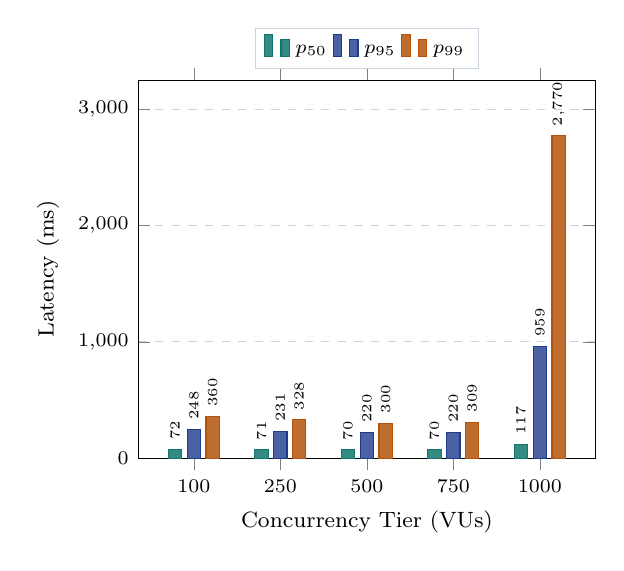
\begin{tikzpicture}
\begin{axis}[
    ybar,
    bar width=4.8pt,
    scale only axis,
    width=5.8cm,
    height=4.8cm,
    ylabel={Latency (ms)},
    symbolic x coords={100, 250, 500, 750, 1000},
    xtick=data,
    xticklabels={100, 250, 500, 750, 1000},
    xlabel={Concurrency Tier (VUs)},
    x tick label style={font=\scriptsize},
    y tick label style={font=\scriptsize},
    label style={font=\footnotesize},
    ymin=0,
    ymax=3250,
    ymajorgrids=true,
    grid style={dashed, color=RuleGray},
    legend style={at={(0.5,1.03)}, anchor=south, legend columns=3, font=\scriptsize, draw=RuleGray},
    enlarge x limits=0.16,
    nodes near coords,
    every node near coord/.append style={font=\tiny, rotate=90, anchor=west}
]
\addplot[fill=TealSignal!85, draw=TealSignal] coordinates {
    (100, 72) (250, 71) (500, 70) (750, 70) (1000, 117)
};
\addplot[fill=BlueAccent!80, draw=BlueAccent] coordinates {
    (100, 248) (250, 231) (500, 220) (750, 220) (1000, 959)
};
\addplot[fill=AmberWarn!85, draw=AmberWarn] coordinates {
    (100, 360) (250, 328) (500, 300) (750, 309) (1000, 2770)
};
\legend{$p_{50}$, $p_{95}$, $p_{99}$}
\end{axis}
\end{tikzpicture}
\end{minipage}
\hfill
\begin{minipage}[b]{0.49\textwidth}
\centering
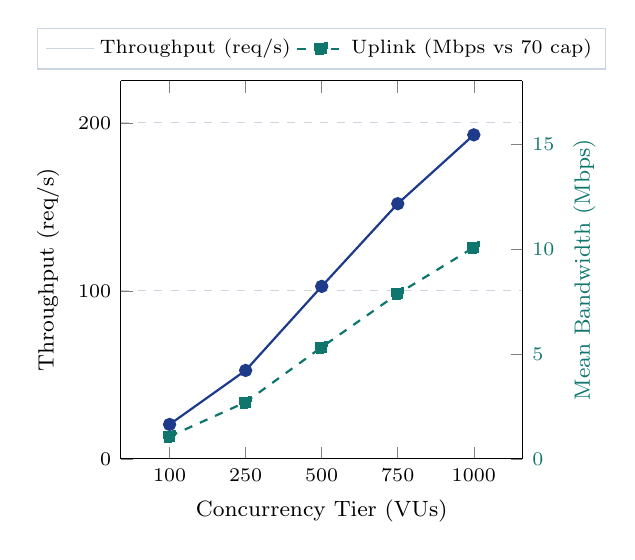
\begin{tikzpicture}
\begin{axis}[
    scale only axis,
    width=5.1cm,
    height=4.8cm,
    xlabel={Concurrency Tier (VUs)},
    ylabel={Throughput (req/s)},
    axis y line*=left,
    symbolic x coords={100, 250, 500, 750, 1000},
    xtick=data,
    xticklabels={100, 250, 500, 750, 1000},
    x tick label style={font=\scriptsize},
    y tick label style={font=\scriptsize},
    label style={font=\footnotesize},
    ymin=0,
    ymax=225,
    enlarge x limits=0.16,
    ymajorgrids=true,
    grid style={dashed, color=RuleGray}
]
\addplot[color=BlueAccent, thick, mark=*, mark size=2pt] coordinates {
    (100, 20.51) (250, 52.66) (500, 102.69) (750, 151.92) (1000, 192.90)
};
\label{plot:rps}
\end{axis}
\begin{axis}[
    scale only axis,
    width=5.1cm,
    height=4.8cm,
    axis y line*=right,
    axis x line=none,
    ylabel={Mean Bandwidth (Mbps)},
    ylabel style={color=TealSignal, font=\footnotesize},
    y tick label style={color=TealSignal, font=\scriptsize},
    symbolic x coords={100, 250, 500, 750, 1000},
    ymin=0,
    ymax=18,
    enlarge x limits=0.16,
    legend style={at={(0.5,1.03)}, anchor=south, legend columns=2, font=\scriptsize, draw=RuleGray}
]
\addlegendimage{/pgfplots/refstyle=plot:rps}\addlegendentry{Throughput (req/s)}
\addplot[color=TealSignal, thick, dashed, mark=square*, mark size=2pt] coordinates {
    (100, 1.07) (250, 2.70) (500, 5.32) (750, 7.86) (1000, 10.07)
};
\addlegendentry{Uplink (Mbps vs 70 cap)}
\end{axis}
\end{tikzpicture}
\end{minipage}
\caption{Five-tier scaling behavior (\texttt{100--1000 VUs}). \textbf{Left:} Latency percentiles stay flat through $750\text{ VUs}$ ($p_{50} \le 72\text{ ms}$, $p_{99} \le 360\text{ ms}$) before inflecting at $1{,}000\text{ VUs}$. \textbf{Right:} Mean throughput and bandwidth scale smoothly to $192.90\text{ req/s}$ ($10.07\text{ Mbps}$, just $14.4\%$ of the $70\text{ Mbps}$ physical link).}
\label{fig:latency_comparison}
\end{figure}

\subsection{Route-Level Performance Profile and Tier-5 Inflection Diagnosis}
Inspecting per-route metrics across all 51 load labels in \texttt{jmeter\_report.pdf} (\texttt{statistics.json} and \texttt{dashboard.js}) paired with raw \texttt{jmeter\_results\_load.jtl} timestamp/connect slicing provides three crisp architectural insights. Table~\ref{tab:slow_routes} reports the highest-$p_{95}$ endpoints alongside fast cached reference/admin endpoints.

\begin{table}[H]
\centering
\caption{Representative route telemetry ordered by $p_{95}$ (\texttt{jmeter\_report.pdf} / \texttt{statistics.json}, $n=22{,}966$ load samples).}
\label{tab:slow_routes}
\scriptsize
\setlength{\tabcolsep}{3pt}
\begin{tabularx}{\textwidth}{@{} >{\raggedright\arraybackslash}X r r r r r r r @{}}
\toprule
\textbf{Endpoint Label (Weight Bucket)} & \textbf{Calls} & \textbf{KB/req} & \textbf{APDEX} & \textbf{$p_{50}$} & \textbf{$p_{95}$} & \textbf{$p_{99}$} & \textbf{Max} \\
\midrule
\texttt{GET /api/events?\_\allowbreak include=...\&\_\allowbreak page=1} (B0) & $894$ & $14.35$ & $0.932$ & $141.0$ & $1003.3$ & $3043.6$ & $5211$ \\
\texttt{GET /api/events?\_\allowbreak sort=eventDate\&\_\allowbreak order=asc} (B0) & $940$ & $14.60$ & $0.932$ & $140.0$ & $994.9$ & $2814.0$ & $6266$ \\
\texttt{GET /api/events?\_\allowbreak page=1\&\_\allowbreak per\_page=10} (B0) & $881$ & $14.35$ & $0.946$ & $140.0$ & $820.6$ & $1944.8$ & $9894$ \\
\texttt{GET /api/bulletins?\_\allowbreak sort=bulletinDate\&\_\allowbreak order=desc} (B0) & $901$ & $12.19$ & $0.960$ & $72.0$ & $812.3$ & $2611.4$ & $5700$ \\
\texttt{GET /api/bulletins?\_\allowbreak page=1\&\_\allowbreak per\_page=10} (B0) & $896$ & $13.39$ & $0.958$ & $71.0$ & $787.4$ & $3227.5$ & $9776$ \\
\texttt{GET /images/engineer.png} (Static Asset, B0) & $905$ & $13.10$ & $0.959$ & $70.0$ & $779.8$ & $2387.1$ & $11986$ \\
\texttt{GET /api/admin/\allowbreak bulletins?\_\allowbreak page=1\&\_\allowbreak per\_page=10} (B3) & $161$ & $13.33$ & $0.963$ & $74.0$ & $739.5$ & $2836.1$ & $3024$ \\
\texttt{GET /api/comments?\_\allowbreak page=1\&\_\allowbreak per\_page=10} (B1) & $339$ & $11.66$ & $0.954$ & $73.0$ & $724.0$ & $3141.0$ & $7130$ \\
\texttt{GET /api/userConnections?\_\allowbreak include=...} (B1) & $353$ & $11.03$ & $0.963$ & $75.0$ & $703.3$ & $1682.7$ & $12491$ \\
\texttt{GET /api/bulletins?\_\allowbreak include=...\&\_\allowbreak page=1} (B0) & $940$ & $13.79$ & $0.968$ & $72.0$ & $688.5$ & $1618.3$ & $5638$ \\
\midrule
\multicolumn{8}{@{}l}{\scriptsize\textit{Representative Fast / Cached Routes in the Same Run (Comparison, latency in ms):}} \\
\texttt{GET /api/admin/dashboard-stats} (B3, $20\text{s}$ Cache) & $149$ & $5.56$ & $0.977$ & $72.0$ & $463.5$ & $1026.0$ & $1136$ \\
\texttt{GET /api/users?\_\allowbreak where=active\&\_\allowbreak include} (B1) & $338$ & $3.80$ & $0.979$ & $73.0$ & $312.4$ & $810.0$ & $4994$ \\
\texttt{GET /api/auth/me [Regular]} (B1) & $349$ & $0.87$ & $0.999$ & $71.0$ & $233.0$ & $407.0$ & $501$ \\
\texttt{GET /api/contentStatuses} (B2, $300\text{s}$ Cache) & $255$ & $0.57$ & $0.988$ & $69.0$ & $210.2$ & $1282.2$ & $1800$ \\
\bottomrule
\end{tabularx}
\end{table}

\begin{enumerate}
  \item \textbf{Flat Sub-360ms Scaling Through 750 VUs \& Bandwidth Validation:} Across Tiers~1 through 4 ($100\text{--}750$ VUs, $14{,}392$ samples), median latency actually tightened slightly ($72.0\to 70.0\text{ ms}$) and $p_{95}$ held inside $220\text{--}248\text{ ms}$ with only $1$ sample above $1500\text{ ms}$. Average paginated event and bulletin payloads dropped to $12.19\text{--}14.60\text{ KB/req}$ ($6.34\text{ KB/req}$ blended across all 51 routes), limiting Tier~5 network consumption to $10.07\text{ Mbps}$ mean ($14.39\%$ of $70\text{ Mbps}$; $15.46\text{ Mbps}$ / $22.1\%$ per-second JTL peak)—confirming zero network-link saturation.
  \item \textbf{Dual Median RTT Strata ($69\text{--}75\text{ ms}$ vs.\ $140\text{--}144.5\text{ ms}$):} Static images, status dictionaries, auth token validations, \texttt{/api/bulletins}, and \texttt{/api/users?\_where=active\&\_include} ($p_{95} = 312.4\text{ ms}$ vs.\ $1935\text{ ms}$ pre-Tier-3) all cluster right on the $\approx 70\text{ ms}$ single-RTT WAN latency floor. By contrast, all paginated \texttt{/api/events} and \texttt{/api/admin/events} samplers settle cleanly one $\approx 70\text{ ms}$ step higher at $p_{50} = 140.0\text{--}144.5\text{ ms}$.
  \item \textbf{Root Cause of Tier~5 Tail Excursion — Transient TLS/Accept Queueing:} Decomposing Tier~5 ($1{,}000$ VUs, $n = 8{,}574$) by JTL \texttt{Connect} times and 1-second windows proves the $959\text{ ms}$ $p_{95}$ and $12{,}491\text{ ms}$ \texttt{Max} did \emph{not} originate from steady-state SQLite read contention:
  \begin{itemize}
    \item Warm keep-alive requests (\texttt{Connect = 0}, $n = 7{,}574$) averaged $257.93\text{ ms}$ ($p_{50} = 97\text{ ms}$, $p_{95} = 895\text{ ms}$). New TLS handshakes (\texttt{Connect > 0}, $n = 1{,}000$) averaged $460.23\text{ ms}$ ($p_{50} = 228\text{ ms}$, $p_{95} = 1548\text{ ms}$), driven by TCP/TLS setup jumping to $\bar{C} = 272.7\text{ ms}$ ($p_{95} = 1{,}126\text{ ms}$, $\max = 9{,}831\text{ ms}$) compared to $140.9\text{--}146.3\text{ ms}$ mean across Tiers~1--4.
    \item Second-by-second slicing pinpoints a transient 9-second window (\texttt{t+206s..t+214s}, i.e.\ $+24\text{--}32\text{ s}$ into Tier~5 as the final ramp cohort pushed active throughput to $252\text{--}284\text{ req/s}$) absorbing the transient $p_{50} = 318\text{--}590\text{ ms}$ / $p_{95} = 1{,}165\text{--}3{,}299\text{ ms}$ queue. Tellingly, even static \texttt{GET /images/engineer.png} (bypassing Node and SQLite via Nginx \texttt{try\_files}) hit $\max = 11{,}986\text{ ms}$ in that exact \texttt{t+208s} window. From \texttt{t+216s} through \texttt{t+225s} at full $1{,}000$-VU concurrency ($248\text{--}312\text{ req/s}$), latency recovered cleanly ($p_{50} = 85\text{--}155\text{ ms}$ except one $233\text{ ms}$ tick; $p_{95} = 261\text{--}679\text{ ms}$; $0$ errors).
  \end{itemize}
  \item \textbf{Workload Scope Boundary:} Because the \texttt{17:41} campaign executed standalone \texttt{run\_jmeter.ps1} without \texttt{-IncludeWritesInLoad} or concurrent Locust writes (the $31$ mutating \texttt{201}/\texttt{204} requests ran sequentially in Phase~1 Coverage), its $0.00\%$ error rate and $0.970$ APDEX certify sustained \textbf{1,000-VU read/cache/TLS capacity}, while concurrent write serialization under \texttt{DELETE} mode continues to be validated via joint \texttt{run\_parallel\_suite.ps1} runs.
\end{enumerate}

% ==============================================================================
% SECTION 8
% ==============================================================================
\section{Operational Governance and Reproducibility}

\subsection{Database Hygiene, Snapshot Recovery, and Rate-Limiter Controls}
Pre-test normalization and post-test cleanup form a strict operational bracket around every campaign against \texttt{dev.db}:
\begin{itemize}
  \item \textbf{Pre-Test Backup \& Provisioning (\texttt{test/load/hell.sql}):} Capture \texttt{cp dev.db dev.db.bak\_pre\_stress\_\$(date +\%s)} before executing \texttt{hell.sql}, especially because Step~6 resets all existing \texttt{UserAuth} and \texttt{Admin} hashes for staging benchmark access.
  \item \textbf{Post-Test Teardown (\texttt{test/load/teardown.sql}):} Automated API \texttt{DELETE} cleanup hooks purge transient Phase~1 and Locust entities; \texttt{teardown.sql} removes remaining synthetic \texttt{loadtest\_\%@najealp.top}, \texttt{test.official\%}, and \texttt{test.regular\%} records followed by \texttt{VACUUM}, or restores original user credentials directly via \texttt{cp dev.db.bak\_pre\_stress\_* dev.db}.
  \item \textbf{Rate-Limit Restoration:} Operators moving from benchmark mode back to public production should confirm whether \texttt{authLimiter} and \texttt{contentLimiter} in \texttt{api/index.js} transition from \texttt{skip: () => true} back to active throttling.
\end{itemize}

\subsection{Standardized Execution Profiles}
Reproducing either the fast DryRun gate, standalone 5-tier JMeter certification (\texttt{jmeter\_report.pdf}), or unified dual-engine write/read testing requires a single PowerShell command from the repository root (with Apache JMeter~5.6.3 and Edge/Chrome installed):
\begin{lstlisting}[language=bash,caption={Reproducible invocation profiles in \texttt{test/load/}.}]
# 1. Fast pre-flight verification & DryRun ([10, 25] VUs x 10s + 20 Locust VUs)
pwsh -NoProfile -ExecutionPolicy Bypass -File test\load\run_parallel_suite.ps1 -DryRun

# 2. Standalone 5-tier JMeter capacity run (reproduces jmeter_report.pdf & .xlsx)
pwsh -NoProfile -ExecutionPolicy Bypass -File test\load\run_jmeter.ps1 -AllReports

# 3. Full joint 5-tier concurrency + Locust write contention suite
pwsh -NoProfile -ExecutionPolicy Bypass -File test\load\run_parallel_suite.ps1
\end{lstlisting}

\begin{calloutbox}[NavyPrimary]{Architectural Status \& Next-Stage Recommendations}
\begin{enumerate}
  \item \textbf{Tier-3 Hardening Empirically Validated:} Switching \texttt{bcryptjs} to async \texttt{await bcrypt.hash}/\texttt{compare}, slimming \texttt{defaultListIncludes}, enabling \texttt{feedCache}/\texttt{lookupCache}/\texttt{adminDashboardStatsCache}, adding $33$ Prisma indexes, and aligning Nginx + Node keep-alive lifted clean multi-hundred-VU capacity to \textbf{$750\text{ VUs}$ at $\text{APDEX} = 0.998$} and \textbf{$1{,}000\text{ VUs}$ with $0.00\%$ HTTP errors ($\text{APDEX} = 0.970$)}.
  \item \textbf{Smooth $1{,}000$-VU Ramp Accept Queues \& Event Feed Latency:} Profile OS/Nginx socket listen backlog (\texttt{somaxconn}, Nginx \texttt{listen ... backlog}, TLS session resumption) to flatten the $+24\text{--}32\text{ s}$ TLS handshake spike during $750\to 1{,}000$-VU ramps, and inspect why \texttt{/api/events} paginated routes sit at $p_{50} = 140\text{ ms}$ ($\approx 2\times$ \texttt{/api/bulletins}'s $71\text{ ms}$).
  \item \textbf{Preserve \texttt{DELETE}-Mode Boundaries via Joint Runs:} Continue honoring \texttt{PRAGMA journal\_mode = DELETE} alongside \texttt{busy\_timeout = 10000}, and re-run \texttt{run\_parallel\_suite.ps1} with concurrent Locust writes after proxy/event-route tuning to certify mixed read/write tail bounds across $500\text{--}1{,}000$ VUs.
\end{enumerate}
\end{calloutbox}

\end{document}
